\chapter{電與磁：同一個相對論性場}

我們已經研究過，給定的電磁場如何使帶電粒子運動。問題尚未完成的另一半是場本身：電場和磁場如何演化，以及電荷和電流如何成為它們的源。麥克斯韋方程組回答了這些問題。不過，在寫出方程之前，值得先回顧那個使其相對論結構成為必然的物理謎題。

這是有意暫時退回形式體系之前。作用量原理稍後會再登場，但不是現在。先從別處開始，是為了在由作用量推導場的動力學之前，先看清楚電場和磁場為什麼必須是同一個物件的組成部分。

\section{愛因斯坦第一段中的謎題}

在比利時訪問期間，一場關於早期索爾維會議的討論，讓話題回到愛因斯坦1905年的論文\emph{《論動體的電動力學》}。論文第一段以驚人的簡潔陳述了其動機。同一個電磁現象，在兩個慣性參考系中竟有兩種看似不同的解釋。一位觀察者稱這個效應是磁的，另一位則稱它是電的。觀察到的運動相同，因此這兩種描述不可能代表兩種不同的物理現象。

這篇論文現在已可用本課程所建立的知識來理解。即使不逐一推演所有計算，開篇段落仍值得一讀，因為它在提出答案之前先問了正確的問題：電的描述和磁的描述可以改變，而物理事件本身如何保持不變？

\subsection{一個電荷、一塊磁體，兩種描述}

設磁場沿\(y\)方向，電荷沿\(x\)軸運動。在實驗室參考系中，電場為零，因此受力是磁力：
\begin{equation}
\mathbf F=q\,\mathbf v\times\mathbf B.
\end{equation}
力指向另一個橫向方向。課堂上快速畫出的座標軸，並非要確定每一個右手定則的正負號；重要的是，力同時垂直於\(\mathbf v\)和\(\mathbf B\)，而且電荷符號反轉時，力的方向也會反轉。

\begin{classroomqa}
\audiencequestion{圖中的力是向上還是向下？}
\lecturerresponse{這取決於電荷的符號。座標軸的取向和\(q\)的符號一旦確定，右手定則就能決定力的方向。就目前的論證而言，重要的只有橫向力確實存在。\lecturetimestamp{00:07:13}}
\end{classroomqa}

愛因斯坦描述的是一條導線，而不是孤立的粒子。原子構成近似固定的晶格，可移動的電荷載子則在其中運動。二十世紀初，觀察導線中的電流也比追蹤單一自由帶電粒子的軌跡容易得多。這裡兩者的差異並不重要：在磁場中運動的載子受到相同的洛倫茲力。

\begin{figure}[H]
\centering
\includegraphics[width=\linewidth]{lecture_08_figure_01.png}
\caption{用來重述愛因斯坦電動力學謎題的運動電荷、橫向磁場與磁體幾何配置。}
\par\smallskip
\textit{課堂時間：00:07:00。}
\end{figure}

現在讓導線或測試電荷保持靜止，改為移動磁體。磁場配置的變化會產生電動勢；用局部的說法來描述，這就是電場。電場沿相同的橫向方向推動靜止電荷。因此，兩種描述分別是
\begin{align}
\text{moving charge, fixed magnet:}\quad&
q\,\mathbf v\times\mathbf B,
\\
\text{fixed charge, moving magnet:}\quad&
q\,\mathbf E'.
\end{align}
相對運動並沒有改變。因此，相對論必須說明：在一個參考系中純粹是磁場的場，為什麼在另一個參考系中會有電場分量。

電與磁不是彼此分離的實體，而是同一個相對論性場中依參考系而異的部分。愛因斯坦當時還沒有現代的場張量記號；在這段文字中，他也沒有把所需的參考系變換稱為洛倫茲變換。儘管如此，變換的問題已經完整地浮現。

\section{電磁場張量}

能同時包含電場與磁場資訊的物件，是反對稱張量
\begin{equation}
F_{\mu\nu}
=
\partial_\mu A_\nu-\partial_\nu A_\mu.
\label{eq:field-tensor-definition}
\end{equation}
希臘指標取遍\(0,1,2,3\)，其中\(x^0=t\)；拉丁指標則取遍三個空間方向。反對稱性
\begin{equation}
F_{\mu\nu}=-F_{\nu\mu},
\end{equation}
使對角元素為零，並留下六個獨立分量。這六個分量恰好是\(\mathbf E\)的三個分量和\(\mathbf B\)的三個分量。

採用度規
\begin{equation}
\eta_{\mu\nu}=\operatorname{diag}(-1,1,1,1),
\end{equation}
以及沿用前一講帶電粒子作用量的慣例，定義
\begin{align}
E_m&=F_{0m}
=\partial_0A_m-\partial_mA_0,
\label{eq:e-from-a}
\\
B_i&=(\boldsymbol\nabla\times\mathbf A)_i.
\label{eq:b-from-a}
\end{align}
講課時在寫第一行公式時修正了一個空間指標。上面的關係式才是正確寫法：等式兩邊的自由空間指標必須一致。

\begin{figure}[H]
\centering
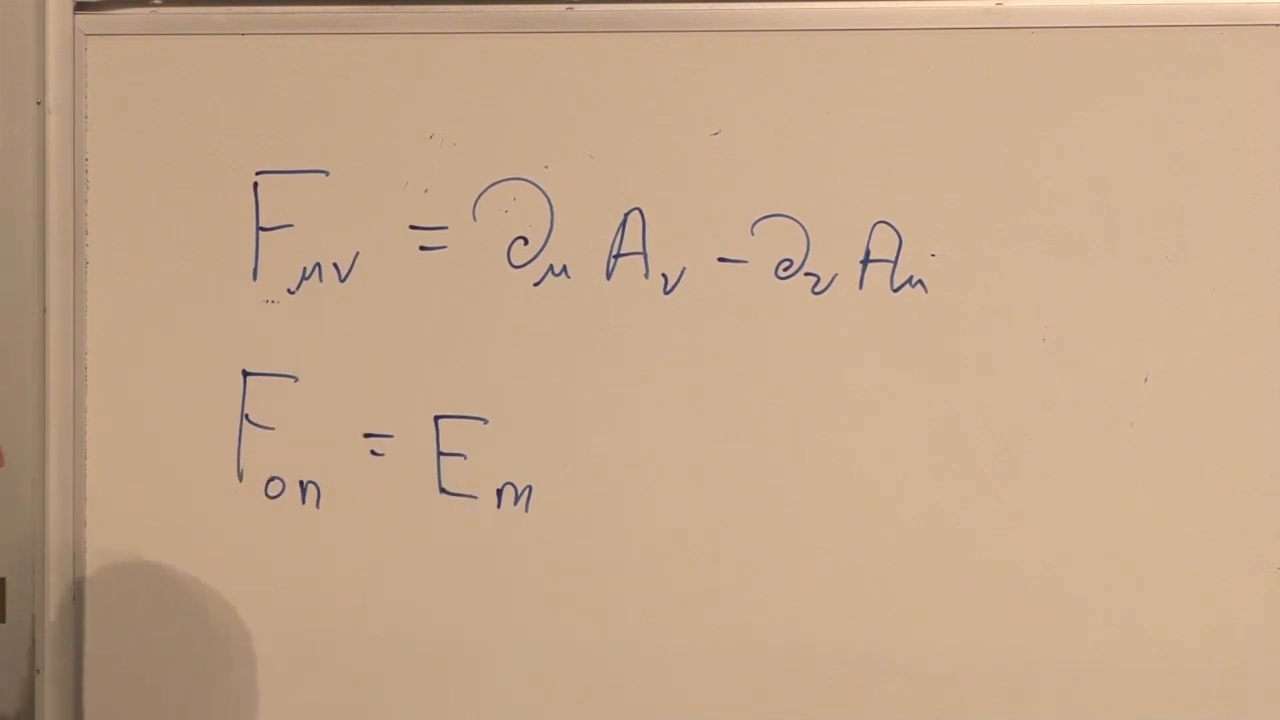
\includegraphics[width=\linewidth]{lecture_08_figure_02.png}
\caption{場張量的定義，以及對應於電場的混合時間--空間分量。}
\par\smallskip
\textit{課堂時間：00:13:15。}
\end{figure}

磁場的關係式來自同一定義的空間部分。例如，
\begin{equation}
B_x
=
\partial_yA_z-\partial_zA_y
=
F_{yz},
\end{equation}
另外兩個分量則由循環置換得到。

\begin{figure}[H]
\centering
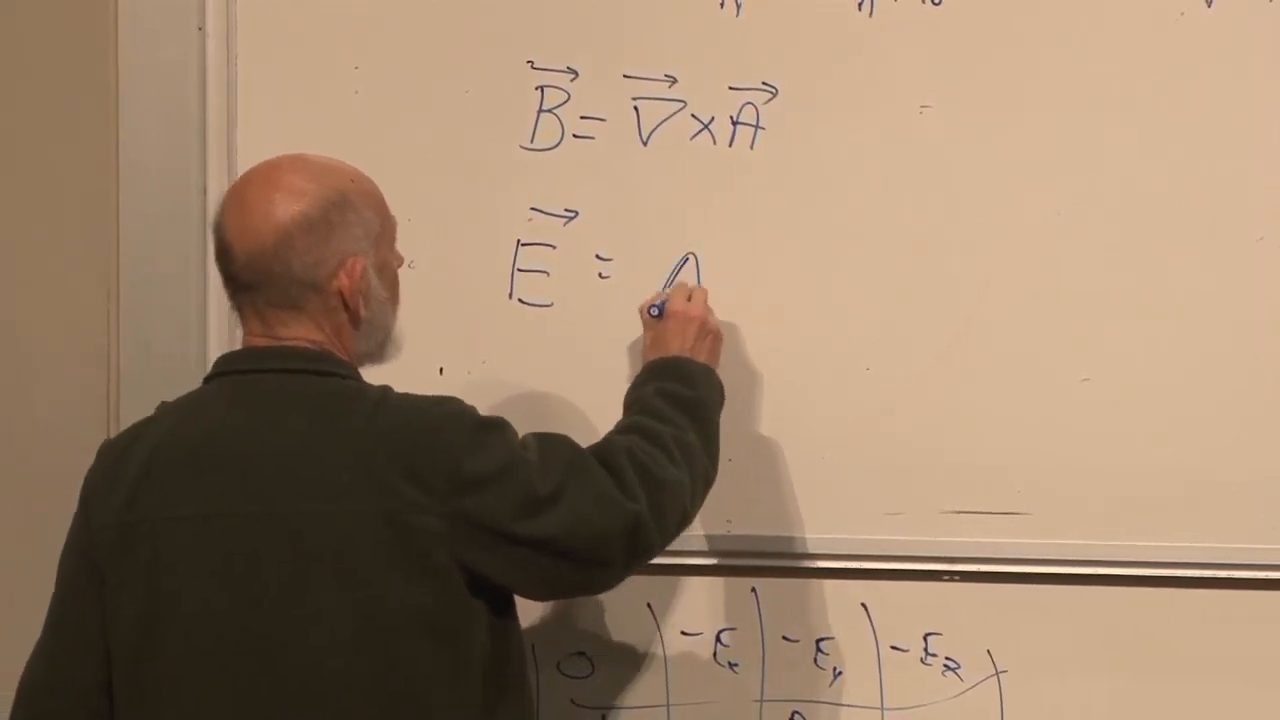
\includegraphics[width=\linewidth]{lecture_08_figure_03.png}
\caption{黑板上列出的電場向量勢公式與磁場旋度公式。}
\par\smallskip
\textit{課堂時間：00:14:00。}
\end{figure}

\subsection{分量矩陣}

令第一個張量指標標示列、第二個指標標示行，並依\(0,x,y,z\)排序。於是
\begin{equation}
F_{\mu\nu}
=
\begin{pmatrix}
0&E_x&E_y&E_z\\
-E_x&0&B_z&-B_y\\
-E_y&-B_z&0&B_x\\
-E_z&B_y&-B_x&0
\end{pmatrix}.
\label{eq:f-lower-matrix}
\end{equation}
混合時間--空間部分包含\(\mathbf E\)；空間\(3\times3\)區塊則包含\(\mathbf B\)。下三角區域不含新資訊，因為它是上三角區域的負轉置。

\begin{figure}[H]
\centering
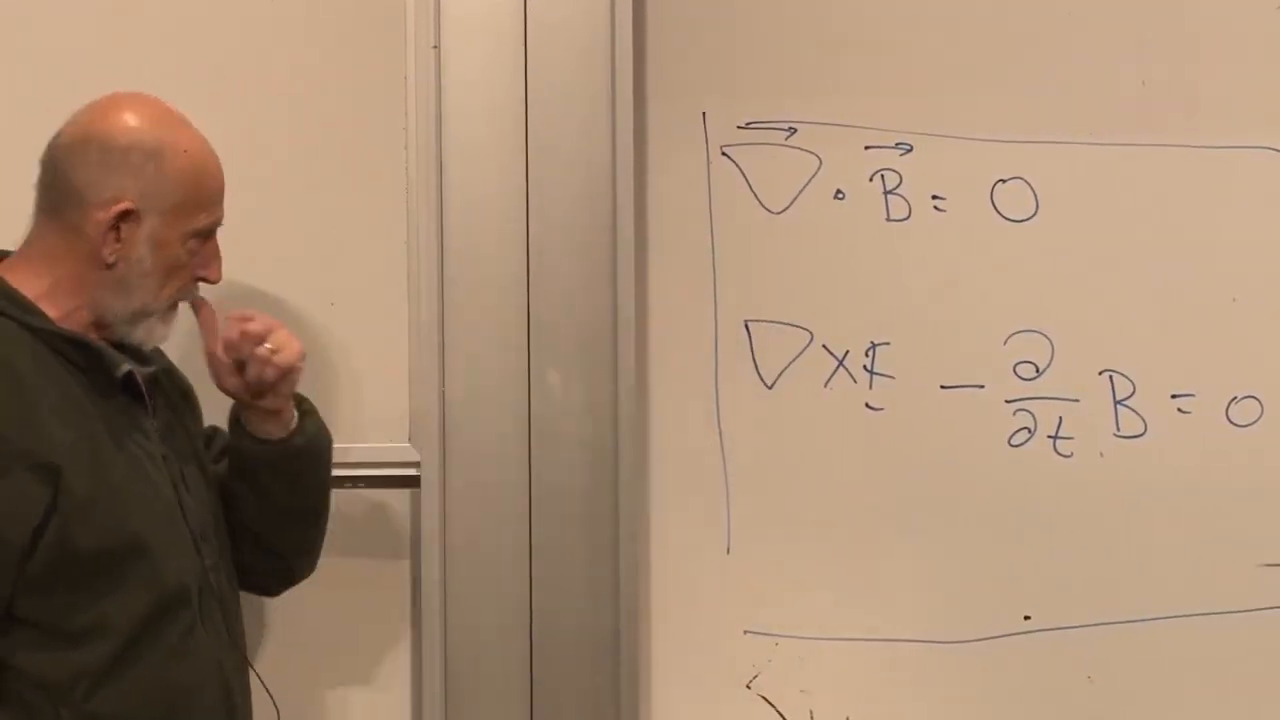
\includegraphics[width=\linewidth]{lecture_08_figure_04.png}
\caption{完整的下標電磁場張量，呈現其電場部分與磁場空間區塊。}
\par\smallskip
\textit{課堂時間：00:17:15。}
\end{figure}

升高兩個指標後，每個電場分量的符號都會改變，磁場分量則保持不變：
\begin{equation}
F^{\mu\nu}
=
\begin{pmatrix}
0&-E_x&-E_y&-E_z\\
E_x&0&B_z&-B_y\\
E_y&-B_z&0&B_x\\
E_z&B_y&-B_x&0
\end{pmatrix}.
\label{eq:f-upper-matrix}
\end{equation}
電場分量帶有一個時間指標，因此會多出一個負號。磁場分量帶有兩個空間指標，因此不會多出負號。

\begin{classroomqa}
\audiencequestion{我對矩陣的理解正確嗎？磁場分量沒有時間指標？}
\lecturerresponse{正確。磁場分量位於純空間區塊。電場分量正是第一列和第一行中的混合時間--空間項。\lecturetimestamp{00:18:55}}
\end{classroomqa}

\section{對純磁場作洛倫茲變換}

考慮沿\(x\)方向的洛倫茲變換，其中\(c=1\)：
\begin{align}
t'&=\gamma(t-vx),
&
x'&=\gamma(x-vt),
&
y'&=y,
&
z'&=z,
\end{align}
其中
\begin{equation}
\gamma=\frac{1}{\sqrt{1-v^2}}.
\end{equation}
寫成矩陣形式為
\begin{equation}
x'^\mu
=
\Lambda^\mu{}_\nu x^\nu,
\qquad
\Lambda^\mu{}_\nu
=
\begin{pmatrix}
\gamma&-\gamma v&0&0\\
-\gamma v&\gamma&0&0\\
0&0&1&0\\
0&0&0&1
\end{pmatrix}.
\label{eq:x-boost}
\end{equation}

\begin{classroomqa}
\audiencequestion{洛倫茲變換矩陣是不是漏了一個負號？}
\lecturerresponse{是的。非對角線上的時間--空間項必須帶有負號，才能符合\(t'=\gamma(t-vx)\)和\(x'=\gamma(x-vt)\)。在用來變換場之前，這個錯誤已經修正。\lecturetimestamp{00:23:50}}
\end{classroomqa}

\begin{figure}[H]
\centering
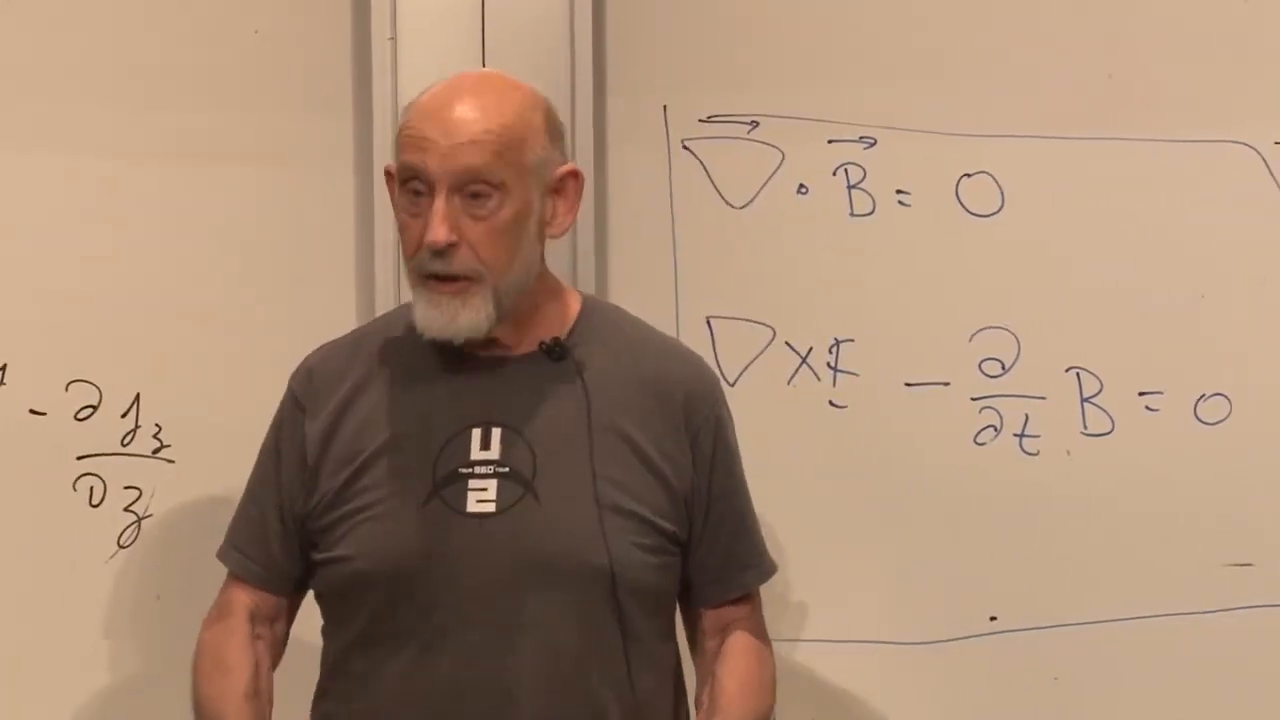
\includegraphics[width=\linewidth]{lecture_08_figure_05.png}
\caption{沿\(x\)軸運動時的修正後洛倫茲變換矩陣。}
\par\smallskip
\textit{課堂時間：00:24:00。}
\end{figure}

張量的每個上標都依照上標向量指標的方式變換。因此
\begin{equation}
F'^{\mu\nu}
=
\Lambda^\mu{}_\sigma
\Lambda^\nu{}_\tau
F^{\sigma\tau}.
\label{eq:f-boost-law}
\end{equation}
重複出現的\(\sigma\)和\(\tau\)是虛指標。張量若有更多指標，就會為每個指標各乘上一個變換矩陣。

\begin{figure}[H]
\centering
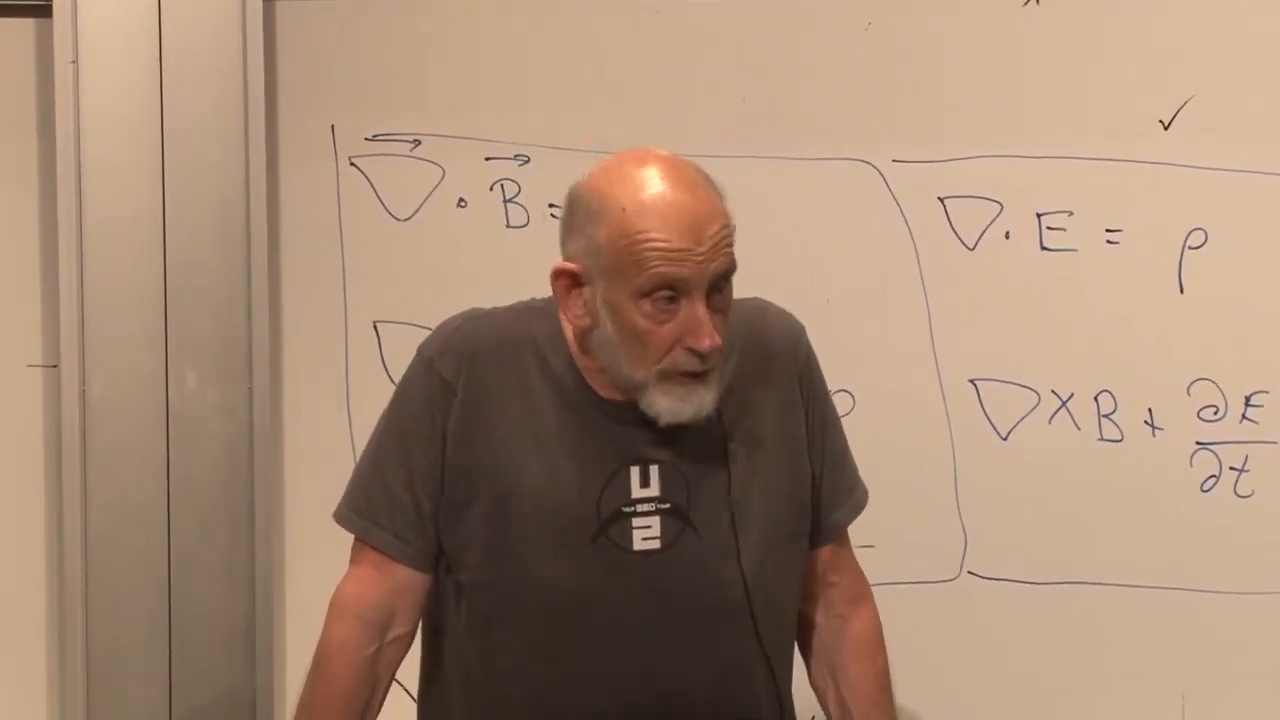
\includegraphics[width=\linewidth]{lecture_08_figure_06.png}
\caption{二階張量的洛倫茲變換律：場張量的每個指標都各自對應一個變換矩陣。}
\par\smallskip
\textit{課堂時間：00:26:40。}
\end{figure}

\subsection{轉換後成為電場的分量}

假設未加撇的參考系中只有磁場\(B_y\)。按照方程式~\eqref{eq:f-upper-matrix}的慣例，相關的獨立分量是
\begin{equation}
F^{xz}=-B_y.
\end{equation}
我們要找的是加撇後的混合分量\(F'^{0z}\)，因為它對應於加撇後電場的\(z\)分量。依據方程式\eqref{eq:f-boost-law}，有
\begin{align}
F'^{0z}
&=
\Lambda^0{}_\sigma
\Lambda^z{}_\tau F^{\sigma\tau}
\\
&=
\Lambda^0{}_x\Lambda^z{}_zF^{xz}
\\
&=
(-\gamma v)(1)(-B_y)
=
\gamma vB_y.
\end{align}
由於在此慣例下\(F'^{0z}=-E'_z\)，
\begin{equation}
E'_z=-\gamma vB_y.
\label{eq:boosted-electric-field}
\end{equation}
符號取決於所指定的座標軸取向與場的慣例；計算中不變的重點是
\begin{equation}
\lvert E'_z\rvert
=
\gamma\lvert vB_y\rvert
\ne0.
\end{equation}
原來的場只有這一個獨立磁場分量，因此雙重求和中的其他項都為零。

\begin{figure}[H]
\centering
\includegraphics[width=\linewidth]{lecture_08_figure_07.png}
\caption{洛倫茲變換後選定的張量分量，其中\(\gamma v\)乘上原來的磁場分量。}
\par\smallskip
\textit{課堂時間：00:32:30。}
\end{figure}

選擇一個隨電荷一起運動的加撇參考系。電荷在這個參考系中靜止，因此其所受力的磁力部分\(q\,\mathbf v'\times\mathbf B'\)為零。然而，力並沒有消失：它是\(q\mathbf E'\)。實驗室觀察者描述的磁力，以及共動觀察者描述的電力，是同一事件的兩種說法。

這就是愛因斯坦第一段所提謎題的答案。這個問題占了本講前約四十分鐘；歷史上的趣談是，它占用愛因斯坦的時間更久。這番計算值得花時間，因為它把「電場與磁場會混合」這句話，化為一個明確的張量分量。

\section{麥克斯韋方程組：恆等式與動力學}

現在從電荷所受的力轉向場方程。下一講會從作用量推導這些方程。這一講先陳述方程，理解它們在邏輯上的兩種不同角色，並將其中由恆等式導出的部分寫成協變形式。

\begin{classroomqa}
\audiencequestion{這些方程不是已經推導過了嗎？}
\lecturerresponse{我們推導過的是帶電粒子在給定電磁場中的運動方程。麥克斯韋方程則是場本身的運動方程，其中包括場對電荷和電流的響應。\lecturetimestamp{00:35:10}}
\end{classroomqa}

\begin{classroomqa}
\audiencequestion{麥克斯韋方程有幾個？}
\lecturerresponse{共有八個純量分量方程。用向量記號可將它們寫成兩個純量方程和兩個三分量向量方程，慣例上稱為四個麥克斯韋方程。\lecturetimestamp{00:35:24}}
\end{classroomqa}

我們繼續採用\(c=1\)的單位制，並將通常的真空常數吸收到電荷和電流的定義中。八個分量方程中，有四個來自定義\(F=dA\)，屬於運動學恆等式。另外四個則是動力學方程；若場的作用量改變，這些方程也可能改變。

\subsection{三種基本向量運算}

對可微的三維向量場\(\mathbf A\)，
\begin{align}
(\boldsymbol\nabla\times\mathbf A)_x
&=
\partial_yA_z-\partial_zA_y,
\\
\boldsymbol\nabla\cdot\mathbf A
&=
\partial_xA_x+\partial_yA_y+\partial_zA_z.
\end{align}
其餘旋度分量可由座標\(x\to y\to z\to x\)作循環置換得到。對純量場\(s\)，
\begin{equation}
\boldsymbol\nabla s
=
(\partial_xs,\partial_ys,\partial_zs).
\end{equation}
因此，旋度是向量，散度是純量，梯度則是向量。

\begin{classroomqa}
\audiencequestion{需要完整複習旋度和散度的定義嗎？}
\lecturerresponse{這裡列出了分量定義，但不必把其餘分量全都展開；循環置換座標標記即可得到它們。\lecturetimestamp{00:37:32}}
\end{classroomqa}

光滑函數的偏導數可以交換次序，因此有以下兩個恆等式：
\begin{align}
\boldsymbol\nabla\cdot
(\boldsymbol\nabla\times\mathbf A)
&=0,
\label{eq:div-curl}
\\
\boldsymbol\nabla\times
(\boldsymbol\nabla s)
&=\mathbf0.
\label{eq:curl-grad}
\end{align}

\begin{classroomqa}
\audiencequestion{我們要不要寫出旋度的散度為零的完整分量證明？}
\lecturerresponse{全班決定不必。展開各分量後會出現\(\partial_x\partial_yA_z\)和\(-\partial_y\partial_xA_z\)這類項；由於偏導數可以交換次序，這些項便會相消。\lecturetimestamp{00:40:13}}
\end{classroomqa}

\begin{figure}[H]
\centering
\includegraphics[width=\linewidth]{lecture_08_figure_08.png}
\caption{利用散度的旋度恆等式和梯度的旋度恆等式，可得麥克斯韋方程組中的一半。}
\par\smallskip
\textit{課堂時間：00:41:40。}
\end{figure}

\subsection{向量勢不會產生磁源}

對方程式~\eqref{eq:b-from-a}取散度，得到
\begin{equation}
\boldsymbol\nabla\cdot\mathbf B
=
\boldsymbol\nabla\cdot
(\boldsymbol\nabla\times\mathbf A)
=0.
\label{eq:div-b-zero}
\end{equation}
這裡沒有用到任何運動方程。這個結果只來自勢的表示法和偏導數的光滑性。

\begin{figure}[H]
\centering
\includegraphics[width=\linewidth]{lecture_08_figure_09.png}
\caption{磁場的散度化為旋度的散度。}
\par\smallskip
\textit{課堂時間：00:43:05。}
\end{figure}

\begin{classroomqa}
\audiencequestion{電場的散度是多少？}
\lecturerresponse{在目前採用的單位制中，它就是電荷密度\(\boldsymbol\nabla\cdot\mathbf E=\rho\)。點電荷是電場線從源向外發散的典型例子。
\lecturetimestamp{00:43:20}}
\end{classroomqa}

在目前這個初階層次上，方程式~\eqref{eq:div-b-zero}表示磁荷密度為零。光滑且在全域定義的向量勢，無法產生磁單極源。稍後必須為這項說法加上限定：磁單極可以用定義於重疊區域上的勢，或帶有奇異性的規範選擇來描述。本講暫且不談這項細節。

\subsection{由電勢推出法拉第方程}

方程式~\eqref{eq:e-from-a}以三維向量記號寫成
\begin{equation}
\mathbf E
=
\frac{\partial\mathbf A}{\partial t}
-\boldsymbol\nabla A_0.
\label{eq:e-vector-potential}
\end{equation}
\(A_0\)是四維向量的一個分量，但在一般的空間旋轉下是純量。對電場取旋度：
\begin{align}
\boldsymbol\nabla\times\mathbf E
&=
\boldsymbol\nabla\times
\frac{\partial\mathbf A}{\partial t}
-
\boldsymbol\nabla\times
(\boldsymbol\nabla A_0)
\\
&=
\frac{\partial}{\partial t}
(\boldsymbol\nabla\times\mathbf A)
\\
&=
\frac{\partial\mathbf B}{\partial t}.
\end{align}
空間旋度運算與時間微分可以交換次序，而梯度的旋度為零。

\begin{figure}[H]
\centering
\includegraphics[width=\linewidth]{lecture_08_figure_10.png}
\caption{黑板上完整呈現磁場旋度、電勢公式，以及旋度計算的起始步驟。}
\par\smallskip
\textit{課堂時間：00:47:45。}
\end{figure}

因此，四個齊次分量方程為
\begin{align}
\boldsymbol\nabla\cdot\mathbf B&=0,
\label{eq:homogeneous-div}
\\
\boldsymbol\nabla\times\mathbf E
-\frac{\partial\mathbf B}{\partial t}
&=\mathbf0.
\label{eq:homogeneous-curl}
\end{align}
第一個是純量方程，第二個則是三分量向量方程。

\begin{figure}[H]
\centering
\includegraphics[width=\linewidth]{lecture_08_figure_11.png}
\caption{直接由勢的定義得到的無源麥克斯韋方程組。}
\par\smallskip
\textit{課堂時間：00:48:45。}
\end{figure}

\subsection{動力學方程}

其餘方程為
\begin{align}
\boldsymbol\nabla\cdot\mathbf E&=\rho,
\label{eq:gauss-electric}
\\
\boldsymbol\nabla\times\mathbf B
+\frac{\partial\mathbf E}{\partial t}
&=-\mathbf J.
\label{eq:ampere-maxwell}
\end{align}
它們不是\(F=dA\)的推論，而是描述源如何產生和改變場；下一講將從電磁作用量推導這些方程。電流項的負號由已選定的慣例決定：\(F_{0i}=E_i\)、\(F_{ij}=\epsilon_{ijk}B_k\)以及\(\partial_\mu F^{\mu\nu}=J^\nu\)。課堂上最初寫出的方程把\(\mathbf J\)放在等號右側，卻漏了這個負號；由此造成的電荷守恆不一致，在下一講才被發現並修正。

\begin{classroomqa}
\audiencequestion{旋度方程右邊是什麼類型的量？}
\lecturerresponse{左邊是三維向量，因此右邊也是三維向量，稱為電流密度\(\mathbf J\)。高斯方程右邊則是三維純量電荷密度\(\rho\)。
\lecturetimestamp{00:50:36}}
\end{classroomqa}

\begin{figure}[H]
\centering
\includegraphics[width=\linewidth]{lecture_08_figure_12.png}
\caption{麥克斯韋四個方程分成兩組：由恆等式導出的方程，以及含源的動力學方程。}
\par\smallskip
\textit{課堂時間：00:50:40。}
\end{figure}

\section{電荷與電流：時空中的流}

現在必須為符號\(\rho\)和\(\mathbf J\)賦予幾何意義。電荷密度是單位體積內的電荷量；電流密度則是單位時間內穿過有向面積的電荷量。本講從世界線出發建立這兩個概念，讓它們之後合為一個四維向量時，不顯得是偶然的拼湊。

\subsection{隔壁黑板引發的課堂插曲}

在畫出那些世界線之前，隔壁教室黑板上可見的方程引出了一段簡短的教學插曲。一門即將開設的課程，將為數學系教師介紹量子力學，讓他們具備學習量子場論及其與現代數學關聯所需的背景知識。這項挑戰是雙向的：物理學家必須把習以為常、未明說的物理觀念講清楚；數學家則必須理解形式架構所要描述的對象。

\begin{classroomqa}
\audiencequestion{誰可能覺得這項教學工作很令人挫折？}
\lecturerresponse{可能雙方都會：物理學家要教不熟悉的聽眾，數學家則要理解形式架構背後的物理觀念。不過，這項工作預期仍會很有趣。接著，課堂回到電荷與電流。\lecturetimestamp{00:53:20}}
\end{classroomqa}

\subsection{電荷密度}

把時間軸畫成垂直方向，其餘畫出的方向代表三維空間。帶電粒子沿著世界線運動。在某個固定時刻，取一個體積為\(\Delta V\)的小空間立方體，讓它截過這束世界線，再將立方體內粒子的電荷加總。電荷密度為
\begin{equation}
\rho(t,\mathbf x)
=
\lim_{\Delta V\to0}
\frac{\Delta Q}{\Delta V}.
\label{eq:charge-density}
\end{equation}
黑板上的二維正方形代表三維立方體；省略一個空間方向，只是因為四維空間無法完整畫在平面黑板上。

\begin{figure}[H]
\centering
\includegraphics[width=\linewidth]{lecture_08_figure_13.png}
\caption{帶電粒子的世界線穿過一個小空間區域，其中\(\rho=\Delta Q/\Delta V\)。}
\par\smallskip
\textit{課堂時間：00:57:20。}
\end{figure}

\subsection{電流密度}

將時空區域側轉。為了定義\(J_x\)，在\(yz\)平面上取一個面積為\(\Delta A_x\)的小窗口，其平面垂直於\(x\)軸。計算在\(\Delta t\)這段時間內，從負\(x\)側穿越到正\(x\)側的淨電荷：
\begin{equation}
J_x
=
\lim_{\Delta A_x,\Delta t\to0}
\frac{\Delta Q_x}{\Delta A_x\,\Delta t}.
\label{eq:jx-window}
\end{equation}
窗口的取向決定正負號。以同樣的方式，取垂直於\(y\)和\(z\)方向的窗口，就能定義\(J_y\)和\(J_z\)。

黑板上的圖確實難以畫清楚：\(yz\)平面上的窗口看起來像天花板上的窗口，而不是牆上的窗口。需要呈現的相關座標軸，比一次能畫出的還多。即使草圖不夠清楚，不變的定義仍毫無歧義。

\begin{classroomqa}
\audiencequestion{圖中的窗口是在天花板上嗎？}
\lecturerresponse{以房間作比喻的話，是的。重要的是，窗口所在的平面垂直於\(x\)方向。面積為\(yz\)的窗口，量度的是穿過它、沿\(x\)方向的電流。\lecturetimestamp{00:59:38}}
\end{classroomqa}

\begin{figure}[H]
\centering
\includegraphics[width=\linewidth]{lecture_08_figure_14.png}
\caption{電荷電流穿過橫向窗口，其中\(J_x=\Delta Q/(\Delta A\,\Delta t)\)。}
\par\smallskip
\textit{課堂時間：01:01:40。}
\end{figure}

\begin{figure}[H]
\centering
\includegraphics[width=\linewidth]{lecture_08_figure_15.png}
\caption{電荷穿過垂直於三個空間軸的窗口，分別定義出三個電流分量。}
\par\smallskip
\textit{課堂時間：01:02:40。}
\end{figure}

這四個量的定義彼此平行。某一瞬間的空間體積是一個垂直於時間軸的超曲面，因此\(\rho\)代表電荷流經時間法向窗口的通量。\(J_i\)則代表電荷流經空間法向窗口的通量。

\begin{classroomqa}
\audiencequestion{這四個數量，是一個代表時間方向的流和三個代表空間方向的流嗎？}
\lecturerresponse{這正是有用的圖像。空間體積相當於垂直於時間軸的窗口；三個橫向面積則是垂直於\(x\)、\(y\)和\(z\)的窗口。這四種通量合在一起。\lecturetimestamp{01:04:14}}
\end{classroomqa}

由此可得逆變四維電流
\begin{equation}
J^\mu
=
(\rho,J_x,J_y,J_z).
\label{eq:four-current}
\end{equation}

\begin{classroomqa}
\audiencequestion{度規在什麼地方發揮作用？這個電流是協變還是逆變？}
\lecturerresponse{依照這裡的定義，\(\rho\)和三個\(J_i\)構成\(J^\mu\)的分量，這是一個上標四維向量，也就是逆變向量。需要\(J_\mu\)時，再用度規降低其指標。協變形式的麥克斯韋方程將說明，為什麼採用上標是自然的。\lecturetimestamp{01:04:48}}
\end{classroomqa}

\section{休息時間的插曲：黑洞附近的訊號}

到了預定的休息時間，問題轉向先前談過的黑洞。這段內容雖然離開了電動力學，卻是課堂上相當深入的一段交流，也展現了同一項思考原則：區分不同觀察者所作的描述。

\begin{classroomqa}
\audiencequestion{如果遠方觀察者看到落入黑洞的物體在視界附近減速，黑洞看起來會不會被所有曾落入其中的物質覆蓋？}
\lecturerresponse{以施瓦西座標時間描述時，經典理論中的落體會漸近地接近視界。可以把陸續落入的物質想成在視界附近逐漸壓縮成一層層物質。但就實際觀測而言，出射訊號會愈來愈延遲、紅移，也愈來愈微弱。以一般局部頻率發出的光，最初以可見光抵達，接著變成紅外線、微波和無線電波，每個光子所帶的能量也愈來愈低。現實中的遠方探測器不可能永遠看到一個明亮而凍結的物體；它會逐漸暗去，最後融入黑暗。
\lecturetimestamp{01:06:11}}
\end{classroomqa}

對落體觀察者來說，自己的時鐘和局部發出的手電筒光都很正常。遠方觀察者的描述之所以不同，是因為頻率和訊號抵達率都受到紅移。在能量和頻寬有限的情況下，實際上總會有一段訊息是最後能被辨識的。

\begin{classroomqa}
\audiencequestion{物體是否會漸近地接近事件視界？}
\lecturerresponse{那是遠方觀察者以施瓦西座標所作的描述。從量子力學的觀點來看，也必須將逐漸變弱的訊號與黑洞本身的霍金輻射區分開來。時間足夠久之後，微弱的紅移訊號在觀測上會被黑洞自身輻射的背景淹沒。\lecturetimestamp{01:09:24}}
\end{classroomqa}

\begin{classroomqa}
\audiencequestion{如果紅移後的波長增長到超過可觀測宇宙的尺度，會怎麼樣？}
\lecturerresponse{在到達那個極限之前很久，訊號在實際上就已經無法觀測。講課中用霍金輻射的量級估算來說明：大約每一個光穿越時間會發出一個典型量子，
\[
t_{\rm cross}\sim\frac{R_s}{c}.
\]
對大黑洞而言，這是極其微弱的輻射；紅移後的落體訊號會遠早於任何宇宙學波長界限，就變得無法探測。\lecturetimestamp{01:09:50}}
\end{classroomqa}

\begin{classroomqa}
\audiencequestion{每個穿越時間大約發出一個量子的速率，在黑洞整個壽命期間都保持固定嗎？}
\lecturerresponse{不會。蒸發中的施瓦西黑洞會收縮，所以穿越時間縮短，霍金溫度升高，輻射因此加快。以瞬時半徑作維度估算仍然有用，但半徑並非常數。相應地，典型的霍金波長會隨蒸發進行而縮短。\lecturetimestamp{01:11:42}}
\end{classroomqa}

休息之後，脫下夾克，我們回到\(\rho\)和\(\mathbf J\)。

\section{電荷的局部守恆}

人們很容易只用下式陳述電荷守恆：
\begin{equation}
\frac{dQ_{\rm universe}}{dt}=0.
\end{equation}
但這種說法太弱了。電荷可以從一間實驗室消失，又瞬間出現在半人馬座{\proseunicodefont α}星，甚至更遠的后髮座星系團，而總電荷仍保持不變。這樣的定律幾乎沒有實驗上的約束力。

更強的說法是局部守恆：一個區域內的電荷，只能透過穿越該區域邊界而改變。在某點周圍放一個小盒子。如果盒內電荷增加，必定有淨電流流入盒內，穿過六個面；如果電荷減少，則必定有淨電流流出盒外。

\subsection{穿過相對兩面的通量}

考慮兩個垂直於\(x\)軸的面。一個面上的向內電流貢獻取自\(x\)的一個位置；對面的貢獻則取自相距一小段距離的位置。兩者的差除以盒子的寬度，極限為
\begin{equation}
-\partial_xJ_x.
\end{equation}
這裡出現負號，是因為正的\(J_x\)定義為沿\(x\)增加的方向流動，而向外通量會使盒內電荷減少。\(y\)面和\(z\)面這一對，同樣分別貢獻\(-\partial_yJ_y\)和\(-\partial_zJ_z\)。因此
\begin{equation}
\frac{\partial\rho}{\partial t}
=
-\partial_xJ_x-\partial_yJ_y-\partial_zJ_z
=
-\boldsymbol\nabla\cdot\mathbf J.
\end{equation}
等價地，
\begin{equation}
\boxed{
\frac{\partial\rho}{\partial t}
+\boldsymbol\nabla\cdot\mathbf J=0
}.
\label{eq:continuity}
\end{equation}

\begin{figure}[H]
\centering
\includegraphics[width=\linewidth]{lecture_08_figure_16.png}
\caption{局部平衡定律\(\dot\rho=-\boldsymbol\nabla\cdot\mathbf J\)，以及展示邊界電流如何導出此定律的小盒子。}
\par\smallskip
\textit{課堂時間：01：20：45。}
\end{figure}

這通常稱為連續性方程。本講偏好稱之為\emph{局域守恆}：連續性可能讓人聯想到數學上的光滑性假設；其物理意義則是，電荷不可能在此處消失、又在別處重新出現，除非兩處之間有電流。

\subsection{為什麼麥克斯威需要位移電流}

方程~\eqref{eq:continuity}並非對麥克斯威方程組額外獨立加入的一條方程。對高斯定律取時間導數，並對安培--麥克斯威定律取散度：
\begin{align}
\frac{\partial\rho}{\partial t}
&=
\boldsymbol\nabla\cdot
\frac{\partial\mathbf E}{\partial t},
\\
-\boldsymbol\nabla\cdot\mathbf J
&=
\boldsymbol\nabla\cdot
(\boldsymbol\nabla\times\mathbf B)
+
\boldsymbol\nabla\cdot
\frac{\partial\mathbf E}{\partial t}
\\
&=
\boldsymbol\nabla\cdot
\frac{\partial\mathbf E}{\partial t}.
\end{align}
因此，兩式的左側相等，得到
\(\partial_t\rho=-\boldsymbol\nabla\cdot\mathbf J\)，恰好就是方程~\eqref{eq:continuity}。從結構上看，關鍵在於\(\mathbf E\)的時間導數，也就是位移電流項，對使散度關係與電荷守恆相容不可或缺。

\begin{classroomqa}
\audiencequestion{我們還沒說明兩個有源麥克斯威方程從何而來，對吧？}
\lecturerresponse{沒有。它們是接下來要處理的動力學目標，下次課會從作用量推導出來。靜磁學中的旋度定律早在麥克斯威之前就已為人所知；麥克斯威在時間相關的情況下所作的關鍵補充，是位移電流。位移電流使場方程與局域電荷守恆相容。\lecturetimestamp{01:23:15}}
\end{classroomqa}

講課中把詳細的散度計算留作練習，但其結論是必然的：麥克斯威方程組要求電荷守恆。

\section{四維電流及其散度}

將方程~\eqref{eq:continuity}寫成分量形式：
\begin{equation}
\frac{\partial\rho}{\partial t}
+
\frac{\partial J_x}{\partial x}
+
\frac{\partial J_y}{\partial y}
+
\frac{\partial J_z}{\partial z}
=0.
\label{eq:continuity-components}
\end{equation}

\begin{figure}[H]
\centering
\includegraphics[width=\linewidth]{lecture_08_figure_17.png}
\caption{將局域電荷守恆展開，可得一個時間導數和三個空間導數。}
\par\smallskip
\textit{講課畫面：01：25：40。}
\end{figure}

根據方程~\eqref{eq:four-current}定義\(J^\mu\)後，這四項可合併為一次縮並：
\begin{equation}
\boxed{\partial_\mu J^\mu=0}.
\label{eq:four-current-conservation}
\end{equation}
\(\partial_\mu\)的下標與\(J^\mu\)的上標縮並，因此結果是洛倫茲純量。幾何視窗的構造已暗示了這個變換律：\(\rho\)和三個電流分量，是同一電荷通量在四個方向上的分量。

\begin{figure}[H]
\centering
\includegraphics[width=\linewidth]{lecture_08_figure_18.png}
\caption{將分量\((\rho,J_x,J_y,J_z)\)組成\(J^\mu\)，再與四維梯度縮並。}
\par\smallskip
\textit{講課畫面：01：27：10。}
\end{figure}

\begin{classroomqa}
\audiencequestion{\(\rho\)的時間導數何時變成偏導數？}
\lecturerresponse{它從一開始就是偏導數。我們固定空間盒子，觀察其中的電荷密度如何隨時間變化。我們並沒有沿著一條運動軌跡追蹤，因此此處的\(\dot\rho\)是指在固定\(x,y,z\)時的\(\partial\rho/\partial t\)。
\lecturetimestamp{01:28:20}}
\end{classroomqa}

\section{齊次方程的協變形式}

我們現在已有所需的各個對象：
\begin{itemize}
\item \(\mathbf E\)和\(\mathbf B\)是反對稱張量\(F_{\mu\nu}\)的六個獨立分量；
\item \(\rho\)和\(\mathbf J\)是\(J^\mu\)的四個分量；
\item 局域守恆則是純量方程
\(\partial_\mu J^\mu=0\)。
\end{itemize}
本講剩下的工作，是將齊次麥克斯威方程組，也就是方程~\eqref{eq:homogeneous-div}和
\eqref{eq:homogeneous-curl}，寫成一個張量方程。

\subsection{循環導數}

答案是
\begin{equation}
\boxed{
\partial_\sigma F_{\nu\tau}
+
\partial_\nu F_{\tau\sigma}
+
\partial_\tau F_{\sigma\nu}
=0
}.
\label{eq:bianchi}
\end{equation}
這三項以循環方式排列導數指標和場張量的兩個指標。通常可簡寫為
\begin{equation}
\partial_{[\sigma}F_{\nu\tau]}=0,
\end{equation}
其中方括號表示反對稱化。

\begin{figure}[H]
\centering
\includegraphics[width=\linewidth]{lecture_08_figure_19.png}
\caption{將齊次麥克斯威方程組合在一起的循環三指標方程。}
\par\smallskip
\textit{講課畫面：01：33：20。}
\end{figure}

\subsection{三個指標皆為空間指標}

令
\begin{equation}
(\sigma,\nu,\tau)=(x,y,z).
\end{equation}
則
\begin{align}
0
&=
\partial_xF_{yz}
+
\partial_yF_{zx}
+
\partial_zF_{xy}
\\
&=
\partial_xB_x+\partial_yB_y+\partial_zB_z
\\
&=
\boldsymbol\nabla\cdot\mathbf B.
\end{align}
因此，方程~\eqref{eq:bianchi}中三個指標皆為空間指標的分量，正是磁場散度為零。

\begin{figure}[H]
\centering
\includegraphics[width=\linewidth]{lecture_08_figure_20.png}
\caption{循環恆等式中三個指標皆為空間指標的分量，化簡為\(\partial_xB_x+\partial_yB_y+\partial_zB_z=0\)。}
\par\smallskip
\textit{講課畫面：01：35：30。}
\end{figure}

\subsection{一個時間指標}

例如，選取
\begin{equation}
(\sigma,\nu,\tau)=(y,x,0).
\end{equation}
則方程~\eqref{eq:bianchi}會將電場分量的兩個空間導數與磁場分量的一個時間導數結合起來：
\begin{equation}
\partial_yF_{x0}
+
\partial_xF_{0y}
+
\partial_0F_{yx}
=0.
\end{equation}
利用方程~\eqref{eq:f-lower-matrix}中的矩陣，這正是
\begin{equation}
\boldsymbol\nabla\times\mathbf E
-\frac{\partial\mathbf B}{\partial t}
=\mathbf0,
\end{equation}
的一個分量，其相對符號由反對稱性決定。選取其他空間指標組合，便會得到另外兩個旋度分量。

\begin{figure}[H]
\centering
\includegraphics[width=\linewidth]{lecture_08_figure_21.png}
\caption{檢查一個時間指標、兩個空間指標的分量，可得到法拉第方程的一個分量。}
\par\smallskip
\textit{講課畫面：01:38:20。}
\end{figure}

也可以直接證明。將方程~\eqref{eq:field-tensor-definition}代入方程~\eqref{eq:bianchi}。會出現六個二階導數項；由於偏導數可交換，這些項會兩兩抵消。這是散度的旋度為零、梯度的旋度為零這兩個恆等式的四維版本。

\begin{classroomqa}
\audiencequestion{Bianchi 這個名字裡有字母 \(h\) 嗎？}
\lecturerresponse{有。這個循環方程就是電磁學的 Bianchi 恆等式，是一種幾何恆等式的特例；廣義相對論中也會出現這類恆等式。其更深層的幾何意義留待日後討論。
\lecturetimestamp{01:40:28}}
\end{classroomqa}

\subsection{為什麼寫出的六十四個分量只包含四個方程}

三個指標各有四種可能的取值，看起來會產生
\(4^3=64\)個方程。反對稱性消除了其中的冗餘：
\begin{itemize}
\item 任意兩個指標若相同，循環表示式便恆等於零；
\item 三個指標若各不相同，交換指標後仍是同一個方程，至多只差一個正負號；
\item 在四維時，只有
\(\binom{4}{3}=4\)個由互不相同指標組成的無序三元組。
\end{itemize}
共有\(24\)個三個指標皆不相同的有序三元組，可分為四組，每組包含六種排列。其餘\(40\)個有序三元組都為零。四個獨立方程包括一個磁場散度方程，以及法拉第方程的三個分量。

\begin{classroomqa}
\audiencequestion{場張量有六個獨立分量，但三指標表示式似乎包含六十四個方程。為什麼最後只剩四個？}
\lecturerresponse{重複的指標使表示式為零；三個不同指標的排列則會重複同一個關係，至多只差一個正負號。因此，看似有六十四個分量，實際上只剩四個獨立方程。
\lecturetimestamp{01:41:58}}
\end{classroomqa}

方程~\eqref{eq:bianchi}明顯具有張量形式，因此是洛倫茲協變的。在單一光滑勢的描述中，它也表示不存在磁荷密度或磁流。本講到此正好抵達界線：有源的動力學方程及其作用量推導，留待下次課討論。

\section{對偶性與磁單極子問題}

最後的問題回到電源與磁源表面上的不對稱性。在真空中，麥克斯威方程組具有電--磁對偶旋轉：
\begin{equation}
\mathbf E\longrightarrow\mathbf B,
\qquad
\mathbf B\longrightarrow-\mathbf E.
\label{eq:duality-quarter-turn}
\end{equation}
這是在以\(\mathbf E\)和\(\mathbf B\)為軸的抽象平面上旋轉九十度，而不是只交換兩者標籤的反射。若電源和磁源同時存在，電四維流與磁四維流也必須同步旋轉。

\begin{figure}[H]
\centering
\includegraphics[width=\linewidth]{lecture_08_figure_22.png}
\caption{總結時的電--磁對偶圖像：在\(E\)-\(B\)平面上旋轉四分之一圈，而非單純互換。}
\par\smallskip
\textit{講課畫面：01:45:00。}
\end{figure}

\begin{classroomqa}
\audiencequestion{如果無源方程在電磁互換下具有對偶性，為什麼電場分量是時間--空間分量，而磁場分量是空間--空間分量？}
\lecturerresponse{在\(F_{\mu\nu}\)中，這種區分取決於參考系；而無源方程允許對偶旋轉。正確的變換是
\(\mathbf E\to\mathbf B\)和
\(\mathbf B\to-\mathbf E\)；若將磁荷納入考量，源電流也要以類似方式旋轉。直接互換會漏掉必要的符號。\lecturetimestamp{01:43:25}}
\end{classroomqa}

\begin{classroomqa}
\audiencequestion{簡潔的張量圖像是否使磁單極子變得毫無意義？}
\lecturerresponse{不是。這表示磁單極子無法用一個在整個空間中都光滑的向量勢來表示。必須改以分區接合勢函數、採用依賴規範的奇異勢，或改用等價的對偶描述。尚未觀測到基本磁單極子；本講也承諾日後再談磁單極子如何納入這套形式架構，而不是在今晚結束時勉強處理這個問題。
\lecturetimestamp{01:45:50}}
\end{classroomqa}

因此，本講在一個明確的界線處結束。相對論解釋了電場與磁場為何會相互混合。勢的定義導出了齊次麥克斯威方程組及其 Bianchi 形式。電荷流成為四維電流，局域守恆則寫成
\(\partial_\mu J^\mu=0\)。剩下的是動力學部分：電磁作用量，以及協變的有源場方程。